\section{Necesidades de Usuario}

Se realizó una encuesta a estudiantes y docentes de la UPP para conocer su percepción sobre el sistema de control de acceso y la posible implementación de reconocimiento facial. Los resultados clave fueron:

\begin{itemize}
    \item El 97.6\% desea un acceso más seguro.
    \item Las opciones preferidas para un nuevo sistema son: credenciales magnéticas (51.2\%), huella digital (41.5\%) y reconocimiento facial (36.6\%).
    \item El 90.2\% estaría dispuesto a proporcionar su imagen para el acceso.
    \item Las principales preocupaciones son la seguridad de la información (53.7\%), errores del sistema (39\%), privacidad de datos (36.6\%) y la incomodidad por grabación (19.5\%).
    \item Necesidades principales: reducción de tiempos de espera (85\%), facilidad de uso (90\%), consulta en tiempo real (72\%) y seguridad y privacidad de datos (68\%).
\end{itemize}

En conclusión, existe una demanda clara por un sistema de acceso más eficiente y seguro. El reconocimiento facial es viable si se prioriza la protección de datos y se informa adecuadamente a los usuarios.

\begin{table}[H]
\centering
\caption{Resumen de Respuestas de la Encuesta}
\begin{tabular}{|p{6cm}|c|}
\hline
\rowcolor[HTML]{CFE2F3}\textbf{Necesidad Identificada} & \textbf{Porcentaje (\%)} \\
\hline
Reducción de tiempos de espera & 85 \\
Facilidad de uso & 90 \\
Consulta en tiempo real & 72 \\
Seguridad y privacidad de datos & 68 \\
\hline
\end{tabular}
\end{table}

\begin{figure}[H]
\centering
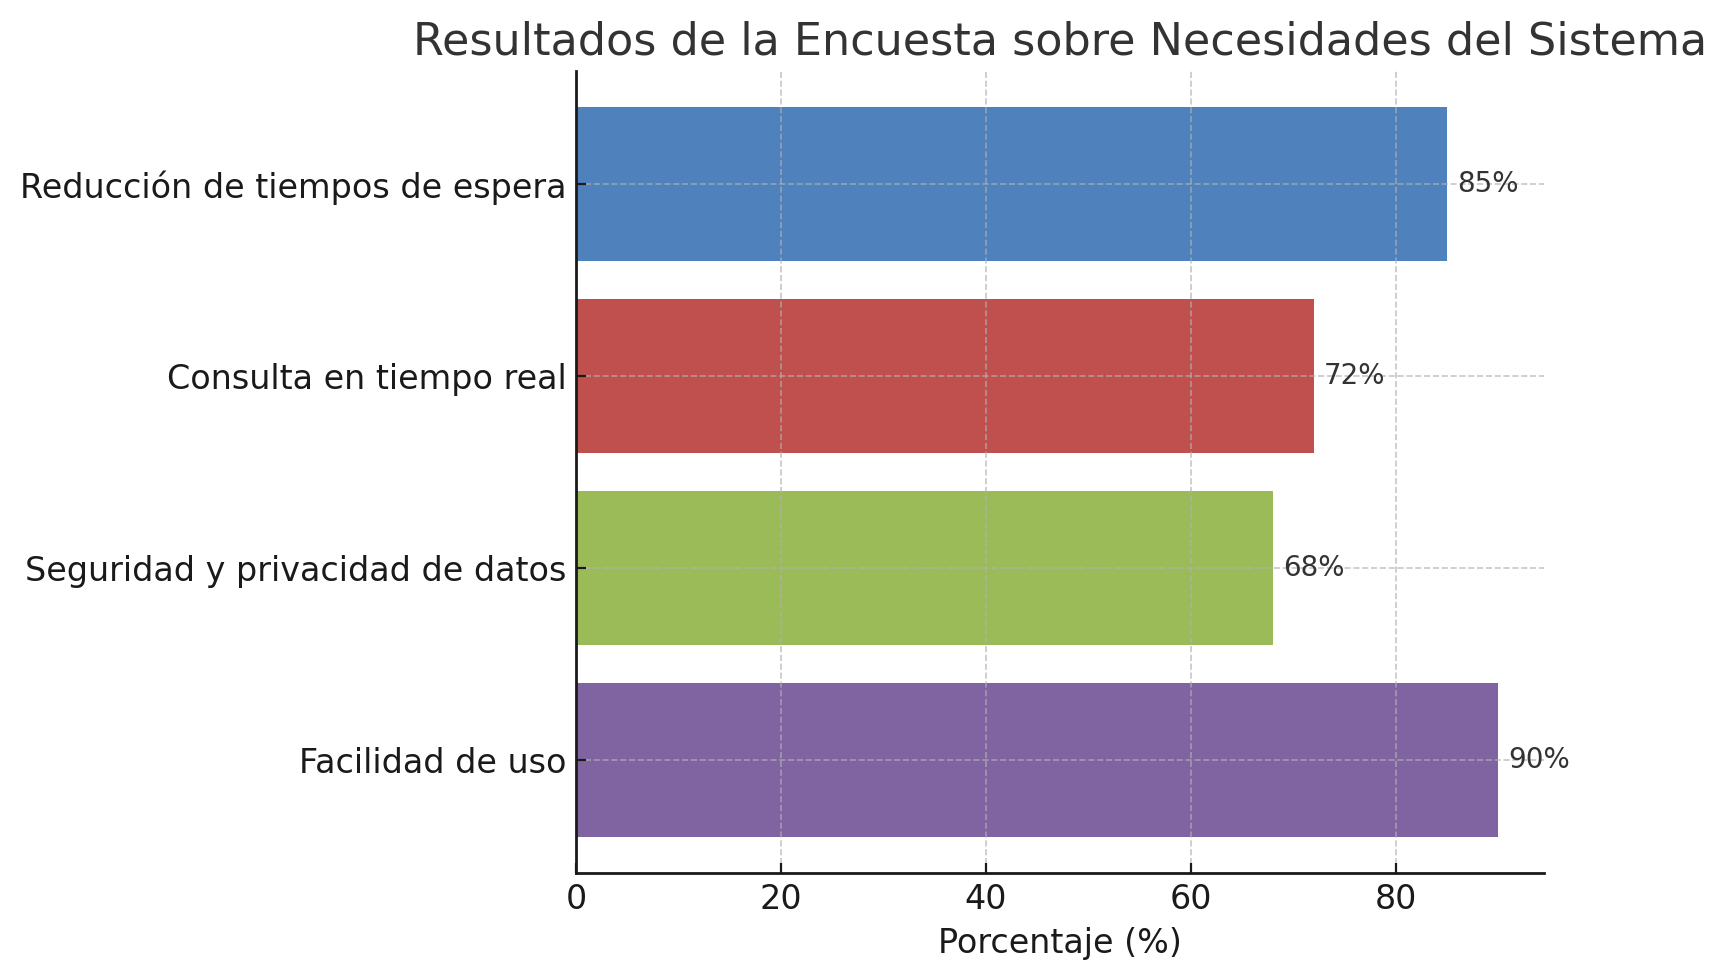
\includegraphics[width=0.8\textwidth]{./Media/grafico_encuesta.png}
\caption{Resultados de la encuesta sobre necesidades del sistema}
\end{figure}